\chapter{Introduction}

\section{Motivation}
Reinforcement Learning is an interesting field of machine learning. An agent learns which
actions to take in an environment given certain rewards. However, the naive algorithms
struggle with high--dimensional sensory input. One way to bypass this problem is the
usage of handcrafted features. These systems are unfortunately not easily applicable
to other problems and highly dependent on the quality of the feature representation. Deep
learning makes it possible to extract higher levels of abstractions from raw sensory input.
These techniques are for example used by Google Deepmind to play seven, and later 49 Atari games with a deep Q--network~\cite{mnih2013playing, mnih2015human}.
Minesweeper is a game almost everyone, who used Microsoft Windows, knows. 
This makes it an interesting subject for a project applying reinforcement learning. Playing
it with a deep reinforcement learning approach enables to learn more in the fields of reinforcement as well as deep learning.

\begin{figure}
	\centering
	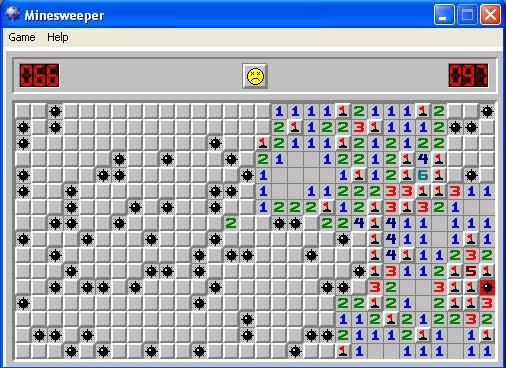
\includegraphics[scale=0.8]{images/img_26041_minesweeper_large.jpg}
	\caption{Minesweeper game played on Windows.}
	\label{fig:minesweeper}
\end{figure}

\section{Minesweeper}
Minesweeper is a video game which was introduced in the $1960$s. 
While Minesweeper looks like an easy game to play, simply checking a board state for consistency is a NP--complete problem.
Deciding which action to take requires logical, arithmetic and as not each decision can be decided by pure logic also probabilistic reasoning.
Human performance is far from optimal~\cite{castillo2003learning}.

The game is represented by equally looking squares that are arranged on a grid. 
Some of the squares contain mines which were randomly assigned at the start of the game. 
At the beginning of every game the grid size as well as the number of mines on the grid is known.
The player can select one of the squares. 
If a square that contains a mine is chosen the game is lost.
Else the square will show a digit from $0$ to $8$.
This digit represents the number of mines that surround the chosen field.
In other words if no field with a mine is adjacent to the chosen one, the chosen one has the digit $0$. 
If all the adjacent squares contain mines the digit will be $8$.
A game is won if all squares without mines are open.
In the original game the player can not only choose to open a square he can also 'flag' or 'unflag' a field.
This means, that if the player is sure that a field contains a mine he can flag it to mark that that field contains a mine.
The flagging is only needed for human players as they are the only way to track mines throughout the game.
The agent does not need a specific way to mark mines with flags and removing this option halves the actions the agent can take.
Additionally we tested the use of flagging in some early games and noticed heavy deadlocking in games.
Flagging a field did not change that much in a state and thus the most probable action after flagging was repeating the same action.
Thus we chose to not have flags as possible actions.

\section{Previous Work}
While Minesweeper is a well--known game, it has not seen much research especially in reinforcement learning.
One paper, that we found is not based on reinforcement learning but instead is based on multirelational learning~\cite{castillo2003learning}.
They use a general purpose learning system (MIO) and use it to learn from examples in clausal logic.
They were able to beat the performance of human players on an $8\times8$ field with $10$ mines.